% !TEX program = xelatex
% WikiBridge 软件设计规格说明书
% 编译：xelatex design_spec.tex 跑两遍（生成目录与图表编号）
\documentclass[UTF8,a4paper,12pt]{ctexart}

\usepackage[margin=2.5cm,headheight=15pt]{geometry}
\usepackage{graphicx}
\usepackage{float}
\usepackage{booktabs}
\usepackage{tabularx}
\usepackage{array}
\usepackage{longtable}
\usepackage{xcolor}
\usepackage{caption}
\usepackage{enumitem}
\usepackage{fancyhdr}
\usepackage{titlesec}
\usepackage{tikz}
\usepackage{hyperref}
\usetikzlibrary{arrows.meta,positioning,fit,calc,shapes.geometric,shapes.multipart,backgrounds}

% ===== 颜色与样式（复用 beamer / uml_architecture 约定）=====
\definecolor{whu}{RGB}{30,55,113}
\definecolor{server}{RGB}{231,239,252}
\definecolor{client}{RGB}{232,248,239}
\definecolor{external}{RGB}{255,246,229}
\definecolor{softgray}{RGB}{246,248,251}

\hypersetup{colorlinks=true, linkcolor=whu, urlcolor=whu, citecolor=whu,
  pdftitle={WikiBridge 软件设计规格说明书}, pdfauthor={WikiBridge 项目组},
  pdfsubject={零代码本地知识库编译与公网发布平台},
  pdfkeywords={WikiBridge, 软件设计规格说明书, 本地知识库, frp, LLM-Wiki}}

% ===== 页眉页脚 =====
\pagestyle{fancy}
\fancyhf{}
\fancyhead[L]{\small WikiBridge 软件设计规格说明书}
\fancyhead[R]{\small V1.0}
\fancyfoot[C]{\thepage}
\renewcommand{\headrulewidth}{0.4pt}
\renewcommand{\footrulewidth}{0pt}

% ===== 章节标题（whu 蓝、贴合 Word「1、」式）=====
\titleformat{\section}{\Large\bfseries\color{whu}}{\thesection、}{0.2em}{}
\titleformat{\subsection}{\large\bfseries\color{whu}}{\thesubsection}{0.6em}{}
\titleformat{\subsubsection}{\normalsize\bfseries\color{whu}}{\thesubsubsection}{0.6em}{}
\titlespacing*{\section}{0pt}{1.2em}{0.6em}
\titlespacing*{\subsection}{0pt}{0.9em}{0.35em}
\titlespacing*{\subsubsection}{0pt}{0.65em}{0.25em}

\newcommand{\keypoint}[1]{\textcolor{whu}{\textbf{#1}}}
\newcommand{\code}[1]{\texttt{#1}}
\newcolumntype{Y}{>{\raggedright\arraybackslash}X}

% 图表按 子节 编号：图 3.1.1 / 图 3.3.2 ...
\counterwithin{figure}{subsection}
\counterwithin{table}{subsection}
\captionsetup{labelsep=quad, font=small, labelfont={bf,color=whu}}
\renewcommand{\thefigure}{\thesubsection.\arabic{figure}}
\renewcommand{\thetable}{\thesubsection.\arabic{table}}

% ===== TikZ 通用样式 =====
\tikzset{
  component/.style={draw=whu, thick, rounded corners=3pt, fill=white, align=center,
    minimum width=3.1cm, minimum height=0.82cm, font=\sffamily\small},
  area/.style={draw=whu, thick, rounded corners=6pt, inner sep=8pt},
  data/.style={draw=whu, thick, cylinder, shape border rotate=90, aspect=0.23, fill=white,
    align=center, minimum height=0.9cm, minimum width=1.8cm, font=\sffamily\small},
  flow/.style={draw=whu, thick, -{Stealth[length=2.2mm]}},
  dashedflow/.style={draw=whu, thick, dashed, -{Stealth[length=2.2mm]}},
  lbl/.style={font=\scriptsize\sffamily, fill=white, inner sep=1pt},
  % 类图
  class/.style={draw=whu, thick, rectangle split, rectangle split parts=3,
    rectangle split draw splits=true, fill=white, align=left,
    font=\scriptsize\sffamily, text width=3.5cm},
  % 时序图
  obj/.style={draw=whu, thick, fill=client, rounded corners=2pt, align=center,
    minimum height=0.72cm, font=\scriptsize\sffamily, inner sep=3pt},
  actor/.style={draw=whu, thick, fill=external, rounded corners=2pt, align=center,
    minimum height=0.72cm, font=\scriptsize\sffamily, inner sep=3pt},
  life/.style={draw=whu, thick, dashed},
  msg/.style={draw=whu, thick, -{Stealth[length=2mm]}},
  ret/.style={draw=whu, thick, dashed, -{Stealth[length=2mm]}},
  slbl/.style={font=\scriptsize\sffamily, midway, above, inner sep=1.5pt},
  % UI 线框
  win/.style={draw=whu, thick, rounded corners=2pt, fill=white},
  bar/.style={draw=whu, thick, fill=server, font=\scriptsize\sffamily},
  el/.style={draw=whu!70, fill=client, rounded corners=1.5pt, font=\scriptsize\sffamily, align=center},
  btn/.style={draw=whu, fill=whu!12, rounded corners=2pt, font=\scriptsize\sffamily, align=center},
  % 部署节点
  node3d/.style={draw=whu, thick, fill=white, align=center, font=\sffamily\small,
    minimum width=4.2cm, minimum height=2.6cm}
}

\begin{document}

% ====================== 封面 ======================
\thispagestyle{empty}
\noindent\small 文档编号：WikiBridge\,--\,SDS\,--\,1.0\hfill\today
\vspace{3cm}

\begin{center}
  {\Huge\bfseries WikiBridge}\\[0.6cm]
  {\LARGE 零代码内网穿透本地知识库平台}\\[1.4cm]
  {\Huge\bfseries 软件设计规格说明书}\\[2.5cm]
  \begin{tikzpicture}
    \node[area, fill=client, minimum width=10cm, align=center, inner sep=14pt]{
      \large
      \begin{tabular}{rl}
        项目名称 & 零代码内网穿透本地知识库平台 WikiBridge\\[4pt]
        文档类型 & 软件设计规格说明书（SDS）\\[4pt]
        开发单位 & 武汉大学 软件工程课程设计 项目组\\[4pt]
        文档版本 & V1.0\\
      \end{tabular}};
  \end{tikzpicture}

  \vfill
  {\large 武汉大学\qquad\today}
\end{center}
\newpage

\pagenumbering{Roman}

% ====================== 变更历史 ======================
\thispagestyle{plain}
\section*{文档变更历史记录}
\addcontentsline{toc}{section}{文档变更历史记录}
\renewcommand{\arraystretch}{1.4}
\begin{tabularx}{\textwidth}{c c c X c}
  \toprule
  \textbf{序号} & \textbf{变更日期} & \textbf{变更人员} & \textbf{变更内容详情描述} & \textbf{版本}\\
  \midrule
  1 & 2026/06/14 & 全员 & 撰写《WikiBridge 软件设计规格说明书》初稿 & V1.0\\
  & & & & \\
  & & & & \\
  \bottomrule
\end{tabularx}
\renewcommand{\arraystretch}{1.0}
\newpage

% ====================== 目录 ======================
\thispagestyle{plain}
\tableofcontents
\newpage

\pagenumbering{arabic}

% ====================== 1 引言 ======================
\section{引言}

\subsection{编写目的}
软件设计过程包括体系结构设计、用户界面设计、用例设计、子系统/构件设计、类设计和数据设计，
分别从不同层次（从宏观到微观、从全局到局部）、不同视角（从结构到行为、从模块到数据）对软件
系统进行设计，产生不同的软件制品（如体系结构模型、用例实现模型、用户界面模型、数据设计模型、
部署模型等）。在完成上述设计工作之后，需要将这些设计成果整合为一个系统、完整的设计方案。本
文档以软件设计规格说明书的形式描述 \keypoint{WikiBridge} 平台的设计方案，方便评审人员对设计
方案的正确性、合理性等方面进行评审，并为后续编码实现提供蓝图。

\subsection{读者对象}
用户、软件设计人员、程序员、软件需求分析人员、质量保证人员、软件测试工程师、配置管理工程师，
以及关注 WikiBridge 平台架构与实现的课程指导教师。

\subsection{软件项目概述}
\begin{itemize}[leftmargin=2.2em]
  \item \textbf{项目名称}：零代码内网穿透本地知识库平台 WikiBridge
  \item \textbf{用户单位}：教师、文字工作者、研究者及中小团队等非技术背景的知识工作者
  \item \textbf{开发单位}：武汉大学 软件工程课程设计 项目组
  \item \textbf{软件项目的背景和大致功能}：
\end{itemize}

在当前数字化学习与办公场景中，个人和小团队会持续积累大量资料——文档、网页剪藏、聊天记录、
课堂笔记、灵感片段等，但它们分散在不同软件与文件夹中，难以长期沉淀，也难以快速找到知识之间
的联系。项目组观察到三类核心痛点：\keypoint{知识零散难归档}、\keypoint{AI 知识库部署门槛高}、
\keypoint{本地知识库共享困难}。现有 RAG 或私有知识库方案通常需要配置 Python 环境、向量数据库、
模型服务甚至 GPU，对非技术用户并不友好；即使在本地搭建了知识库，也很难安全、低成本地发布到
公网供他人访问。

WikiBridge 的目标不是单纯“做一个知识库”，而是让普通用户能够\keypoint{零代码}完成从资料整理、
知识结构化到公网访问的完整闭环。平台将知识库生成过程类比为“软件编译”：用户把原始资料放入本地
素材目录，主动触发 \keypoint{Compile}，系统调用大模型 Agent 对素材进行阅读、提炼、去重与结构化，
输出带有双向链接（\code{[[wiki-links]]}）的 Markdown Wiki；本地 Wiki 经轻量 Web 服务渲染为静态站点，
再借助 \keypoint{frp} 隧道将本地站点映射到公网；外部访问者通过浏览器浏览知识图谱，并可使用 Chatbox
进行问答。其核心优势在于：用户数据与主要计算过程留在本地，云端只负责账号、鉴权、端口和流量调度，
不保存用户知识内容，从而兼顾低成本、隐私性与易用性。

\subsection{文档概述}
本文档主要包含两部分内容：
\begin{enumerate}[leftmargin=2.2em]
  \item \textbf{软件设计约束部分}：包括软件设计目标和原则、软件设计受到的约束和限制。
  \item \textbf{软件设计部分}：主要分为软件体系结构设计、用户界面设计、用例设计、类设计、
        数据设计以及部署设计。
\end{enumerate}

\subsection{定义}
\begin{longtable}{>{\bfseries}p{3.2cm} p{11.2cm}}
  \toprule
  术语 & 含义\\
  \midrule\endhead
  Add & 素材箱管理阶段，用户将原始资料放入本地 \code{/raw} 目录。\\
  Compile & 本地知识编译阶段，调用 LLM Agent 将 \code{/raw} 素材重构为结构化 Markdown Wiki，写入 \code{/wiki}。\\
  Lint & 图谱检查与维护阶段，扫描 \code{/wiki}，修复死链接、孤立页面与冗余结构。\\
  Publish & 无感公网发布阶段，将本地静态站经 frp 隧道映射为可访问的公网 URL。\\
  LLM Agent & 大语言模型“知识主编”，负责素材阅读、实体提取、去重合并与页面生成。\\
  wiki-links & 形如 \code{[[概念]]} 的双向链接，用于在 Wiki 页面之间建立可跳转的知识关联。\\
  frp / frpc / frps & 开源内网穿透工具 frp；frpc 为客户端，运行在用户端；frps 为服务端，运行在云服务器。\\
  控制面 / 数据面 & 控制面指账号、鉴权、端口与隧道调度；数据面指用户的知识内容。WikiBridge 将二者隔离。\\
  \bottomrule
\end{longtable}

\subsection{参考资料}
\begin{enumerate}[leftmargin=2.4em]
  \item 软件工程. 齐治昌, 谭庆平, 宁洪. 北京: 高等教育出版社, 2012.
  \item 需求分析与设计. 马素霞译. 北京: 机械工业出版社, 2009.
  \item 面向使用的软件设计. 刘正捷译. 北京: 机械工业出版社, 2011.
  \item fatedier. frp —— A fast reverse proxy. \url{https://github.com/fatedier/frp}.
  \item WikiBridge 项目简介文档（\code{doc.md}）, 武汉大学软件工程课程设计项目组, 2026.
\end{enumerate}

% ====================== 2 软件设计约束 ======================
\section{软件设计约束}

\subsection{软件设计目标和原则}
软件设计的目标是，根据软件系统的需求（包括功能性需求和非功能性需求），综合考虑软件开发过程中
的各种制约因素（如技术、资源、进度等），遵循软件工程的设计原则（如模块化、信息隐藏、问题分解
等），给出软件系统的实现解决方案和蓝图，产生可指导编码实现的设计模型及文档。具体而言，
WikiBridge 的设计遵循以下策略和原则：
\begin{enumerate}[leftmargin=2.4em]
  \item 抽象和逐步求精的原则；
  \item 模块化与高内聚度、低耦合度的原则——\keypoint{知识编译模块与 frp 隧道管理模块保持解耦}；
  \item 信息隐藏的原则；
  \item 多视点以及关注点分离的原则——\keypoint{控制面与数据面分离}；
  \item 软件重用的原则——复用开源 frp、Markdown 渲染器与 LLM 接口；
  \item 迭代设计的原则；
  \item 可追踪性的原则——设计制品可追溯到需求用例。
\end{enumerate}

\subsection{软件设计的约束和限制}
\begin{itemize}[leftmargin=2.2em]
  \item \textbf{运行环境要求}：用户端为桌面图形界面应用（Windows / macOS / Linux）；服务器端运行
        于 Linux 云主机；知识消费端为现代浏览器，无需安装任何软件。
  \item \textbf{开发语言}：网络隧道改造基于 Go（frp）；知识编译器与本地服务基于 Python / Node.js；
        用户端 GUI 与消费端 Web 前端基于跨平台桌面框架与 HTML/CSS/JavaScript。
  \item \textbf{标准规范}：遵循 RESTful API 设计规范、Markdown / CommonMark 文本规范、
        OpenAI 兼容的对话接口规范。
  \item \textbf{外部依赖}：开源 frp 隧道、可配置的大语言模型服务（API）、Markdown 静态站渲染器。
  \item \textbf{隐私约束}：云端服务器\keypoint{不得存储}用户笔记、文档、Wiki 页面或向量数据，
        用户业务数据主要保留在本地。
\end{itemize}

% ====================== 3 软件设计 ======================
\section{软件设计}

\subsection{软件体系结构设计}
WikiBridge 系统整体分为\keypoint{服务器}、\keypoint{用户端}、\keypoint{用户的用户（知识消费端）}
三个端。服务器承担“控制面”职责——用户认证、Token 鉴权、动态端口/子域名分配、frps 隧道管理与流量
统计，但\keypoint{不保存}用户知识内容；用户端是知识拥有者使用的核心软件，运行知识编译逻辑、本地
Web 服务与网络隧道客户端，对用户屏蔽技术细节；知识消费端无需安装软件，通过浏览器访问公网 URL，
浏览静态 Wiki 并使用 Chatbox 问答。系统总体架构见图~\ref{fig:arch}。

\begin{figure}[H]
  \centering
  \resizebox{\textwidth}{!}{%
  \begin{tikzpicture}[font=\sffamily\scriptsize,
      archbox/.style={component, minimum width=3.6cm, minimum height=1.0cm, inner sep=3pt},
      archdata/.style={data, minimum width=3.4cm, minimum height=1.15cm, inner sep=3pt},
      archlbl/.style={font=\tiny\sffamily, fill=white, inner sep=1pt}]
    \node[archbox, minimum width=3.8cm] (gui) at (0,2.35) {GUI 软件\\部署/发布控制台};
    \node[archbox, minimum width=4.15cm] (kbserver) at (0,0.75) {知识库 Server\\编译/渲染/问答 API};
    \node[archdata] (localdata) at (0,-0.9) {本地素材 /raw\\Wiki /wiki};
    \node[archbox, minimum width=3.8cm] (frpc) at (0,-2.7) {魔改 frpc\\隧道配置与连接};

    \node[archbox, minimum width=3.75cm] (panel) at (7.3,1.9) {管理面板\\用户/发布记录};
    \node[archbox, minimum width=3.75cm] (api) at (7.3,0.35) {管理 API\\端口分配/鉴权};
    \node[archbox, minimum width=3.75cm] (frps) at (7.3,-1.2) {frps 服务\\公网入口};
    \node[archdata, minimum width=3.3cm] (serverdb) at (7.3,-2.95) {用户与端口\\状态数据};

    \node[archbox, minimum width=3.75cm] (kbclient) at (14.2,1.0) {Wiki 浏览\\访问公开入口};
    \node[archbox, minimum width=3.75cm] (chatbox) at (14.2,-0.8) {ChatBox\\对话式问答};

    \begin{scope}[on background layer]
      \node[area, fill=client, inner sep=14pt, fit=(gui)(kbserver)(localdata)(frpc)] (clientarea) {};
      \node[area, fill=server, inner sep=14pt, fit=(panel)(api)(frps)(serverdb)] (serverarea) {};
      \node[area, fill=external, inner sep=14pt, fit=(kbclient)(chatbox)] (externalarea) {};
    \end{scope}
    \node[anchor=south west, text=whu, font=\bfseries] at ([yshift=1pt]clientarea.north west) {用户端};
    \node[anchor=south west, text=whu, font=\bfseries] at ([yshift=1pt]serverarea.north west) {服务器（控制面）};
    \node[anchor=south west, text=whu, font=\bfseries] at ([yshift=1pt]externalarea.north west) {用户的用户};

    \draw[flow] (gui) -- node[archlbl, right, pos=0.48] {启动/配置} (kbserver);
    \draw[flow] (kbserver) -- node[archlbl, right, pos=0.35] {读取/编译} (localdata);
    \draw[flow] (gui.west) -- ++(-0.65,0) |- node[archlbl, pos=0.72, left] {生成隧道配置} (frpc.west);
    \draw[dashedflow] (gui.east) -- node[archlbl, above, pos=0.58] {登录、申请端口、发布} (api.west);
    \draw[flow] (api.east) -- ++(0.48,0) |- node[archlbl, pos=0.65, right] {写入权限和状态} (serverdb.east);
    \draw[flow] (panel) -- node[archlbl, right] {管理操作} (api);
    \draw[flow] (api) -- node[archlbl, right] {配置约束} (frps);
    \draw[flow] (frpc.east) -- node[archlbl, above] {frp 隧道} (frps.west);
    \draw[flow] (frps.east) -- node[archlbl, above, pos=0.55] {公网访问入口} (kbclient.west);
    \draw[flow] (frps.east) -- node[archlbl, below, pos=0.55] {OpenAI 兼容/HTTP} (chatbox.west);

    \node[draw=orange!80!black, fill=external, rounded corners=3pt, align=center,
      minimum width=14.4cm, font=\sffamily\scriptsize] at (7.1,-4.85)
      {架构原则：知识库服务与 frp 管理面板独立演进，通过发布 API、端口权限和隧道配置进行定制化联动。};
  \end{tikzpicture}}
  \caption{WikiBridge 系统的总体体系结构图}
  \label{fig:arch}
\end{figure}

\noindent\textbf{（1）用户端子系统}\quad 用户端采用经典三层结构（见图~\ref{fig:client-layer}）。
界面层提供素材箱、编译控制台、Lint 报告与发布面板；业务逻辑层由 \code{CompileManager}、
\code{LintManager}、\code{PublishManager} 等控制类驱动 Add/Compile/Lint/Publish 工作流；基础服务层
封装 LLM 客户端、本地 Web Server 与魔改 frpc。该子系统依赖服务器的管理 API 获取发布入口。

\begin{figure}[H]
  \centering
  \resizebox{0.96\textwidth}{!}{%
  \begin{tikzpicture}[font=\sffamily\small,
      cbox/.style={component, minimum width=3.05cm}]
    % 界面层 (y=3) / 业务逻辑层 (y=1) / 基础服务层 (y=-1)，四列 x=0,3.6,7.2,10.8
    \node[cbox, fill=client] (ui1) at (0,3)    {素材箱 UI};
    \node[cbox, fill=client] (ui2) at (3.6,3)  {编译控制台 UI};
    \node[cbox, fill=client] (ui3) at (7.2,3)  {Lint 报告 UI};
    \node[cbox, fill=client] (ui4) at (10.8,3) {发布面板 UI};

    \node[cbox, fill=server] (b1) at (0,1)    {AuthClient};
    \node[cbox, fill=server] (b2) at (3.6,1)  {CompileManager};
    \node[cbox, fill=server] (b3) at (7.2,1)  {LintManager};
    \node[cbox, fill=server] (b4) at (10.8,1) {PublishManager};

    \node[cbox] (s1) at (0,-1)    {LLM Agent Client};
    \node[cbox] (s2) at (3.6,-1)  {WikiRepository};
    \node[cbox] (s3) at (7.2,-1)  {Local Web Server};
    \node[cbox] (s4) at (10.8,-1) {魔改 frpc};

    \begin{scope}[on background layer]
      \node[area, fill=client!55, fit=(ui1)(ui4)] {};
      \node[area, fill=server!55, fit=(b1)(b4)] {};
      \node[area, fill=softgray, fit=(s1)(s4)] {};
    \end{scope}

    \node[font=\bfseries\footnotesize, text=whu, rotate=90] at (-2.2,3)  {界面层};
    \node[font=\bfseries\footnotesize, text=whu, rotate=90] at (-2.2,1)  {业务逻辑层};
    \node[font=\bfseries\footnotesize, text=whu, rotate=90] at (-2.2,-1) {基础服务层};

    % 层间依赖（两道居中向下箭头）
    \draw[flow, line width=1pt] (5.4,2.25) -- node[lbl]{调用 / 依赖} (5.4,1.75);
    \draw[flow, line width=1pt] (5.4,0.25) -- node[lbl]{调用 / 依赖} (5.4,-0.25);
  \end{tikzpicture}}
  \caption{“用户端”子系统的分层设计架构}
  \label{fig:client-layer}
\end{figure}

\noindent\textbf{（2）服务器子系统}\quad 服务器只承担控制面职责（见图~\ref{fig:server-layer}）。
\code{AuthController} 负责注册/登录/Token 校验；\code{TunnelController} 与 \code{FrpsManager} 负责动态
分配子域名或端口、维护 frps 与 frpc 的连接状态；\code{TrafficMonitor} 统计带宽、连接时长并实施限速；
所有状态写入控制面数据库（用户、Token、隧道、发布记录），\keypoint{与用户知识内容物理隔离}。

\begin{figure}[H]
  \centering
  \begin{tikzpicture}[font=\sffamily\footnotesize, node distance=0.75cm and 0.85cm,
      srvbox/.style={component, text width=3.0cm, minimum width=3.25cm, minimum height=0.95cm},
      srvdata/.style={data, text width=3.7cm, minimum width=4.5cm, minimum height=1.25cm}]
    \node[srvbox, fill=server] (auth) {AuthController\\认证 / Token};
    \node[srvbox, fill=server, right=of auth] (tun) {TunnelController\\端口/子域名分配};
    \node[srvbox, fill=server, right=of tun] (traf) {TrafficMonitor\\限速 / 统计};
    \node[srvbox, below=1.55cm of tun, text width=4.1cm, minimum width=4.6cm] (frps) {FrpsManager（frps 服务）\\公网入口与连接维护};
    \node[srvdata, below=1.35cm of frps] (db) {控制面数据库\\User / Token / Tunnel};
    \begin{scope}[on background layer]
      \node[area, fill=server!40, inner sep=12pt, fit=(auth)(tun)(traf)] (apilayer) {};
    \end{scope}
    \node[anchor=south west, text=whu, font=\bfseries] at ([yshift=2pt]apilayer.north west) {管理 API 层};

    \draw[flow] (auth) -- (frps);
    \draw[flow] (tun) -- (frps);
    \draw[flow] (traf) -- (frps);
    \draw[flow] (auth.south) -- ++(0,-0.35) -| (db.west);
    \draw[flow] (frps) -- (db);
    \draw[dashedflow] ([xshift=-1.4cm]frps.west) -- node[lbl,above]{frpc 连接} (frps.west);
  \end{tikzpicture}
  \caption{“服务器（控制面）”子系统的设计架构}
  \label{fig:server-layer}
\end{figure}

\subsection{用户界面设计}
根据 WikiBridge 的用例描述及交互流程，用户端 GUI 需要以下一组界面：
\begin{itemize}[leftmargin=2.2em]
  \item 欢迎/引导界面 \code{GuidingUI}：介绍系统用途与“数据本地优先”的隐私边界，引导用户进入工作台。
  \item 登录界面 \code{LoginUI}：输入平台账号并登录，登录后自动申请公网映射。
  \item 素材箱界面 \code{MaterialBoxUI}：管理 \code{/raw} 目录，支持拖拽导入未处理资料。
  \item 编译控制台界面 \code{CompileConsoleUI}：触发 Compile，展示实时进度、日志与错误。
  \item Lint 报告界面 \code{LintReportUI}：触发“检查优化”，展示死链接、孤立页面与冗余结构。
  \item 发布面板界面 \code{PublishPanelUI}：展示本地服务状态、隧道状态与公网访问 URL。
\end{itemize}
知识消费端则包含 \code{WikiBrowseUI}（静态图谱浏览与双向链接跳转）与 \code{ChatboxUI}（上下文问答与
引用展示）。各界面之间的跳转关系见图~\ref{fig:ui-nav}。

\begin{figure}[H]
  \centering
  \begin{tikzpicture}[font=\sffamily\small, node distance=0.55cm and 1.0cm,
      ui/.style={draw=whu, thick, rounded corners=3pt, fill=client, align=center,
        minimum width=2.5cm, minimum height=0.8cm, font=\scriptsize\sffamily}]
    \node[ui] (login) {登录 UI};
    \node[ui, right=of login] (mat) {素材箱 UI};
    \node[ui, right=of mat] (comp) {编译控制台 UI};
    \node[ui, right=of comp] (lint) {Lint 报告 UI};
    \node[ui, right=of lint] (pub) {发布面板 UI};
    \draw[flow] (login) -- node[lbl,above]{登录成功} (mat);
    \draw[flow] (mat) -- node[lbl,above]{Add 完成} (comp);
    \draw[flow] (comp) -- node[lbl,above]{Compile} (lint);
    \draw[flow] (lint) -- node[lbl,above]{Publish} (pub);
    \draw[flow] (comp.south) to[out=-60,in=-120] node[lbl,below]{返回} (mat.south);
    \draw[flow] (pub.north) to[out=60,in=120] node[lbl,above]{再次编译} (comp.north);

    \node[ui, fill=external, below=1.6cm of comp] (wiki) {Wiki 浏览 UI};
    \node[ui, fill=external, right=1.4cm of wiki] (chat) {Chatbox UI};
    \draw[flow] (wiki.east) to[out=20,in=160] node[lbl,above]{提问} (chat.west);
    \draw[flow] (chat.south) to[out=-160,in=-20] node[lbl,below]{引用来源跳转} (wiki.south);
    \draw[dashedflow] (pub) -- node[lbl,right]{分享公网 URL} (chat);
    \node[font=\bfseries\footnotesize,text=whu] at ($(wiki)!0.5!(chat)+(0,0.9)$){消费端（浏览器）};
  \end{tikzpicture}
  \caption{用户界面跳转关系图}
  \label{fig:ui-nav}
\end{figure}

\noindent 下面给出若干关键界面的线框设计。图~\ref{fig:ui-compile} 为“素材箱 + 编译控制台”界面，
左侧管理 \code{/raw} 素材列表，右侧展示编译进度与实时日志。

\begin{figure}[H]
  \centering
  \begin{tikzpicture}[font=\sffamily]
    \node[win, minimum width=12cm, minimum height=6.4cm] (w) at (0,0){};
    \node[bar, minimum width=12cm, minimum height=0.5cm, anchor=north] at (w.north){\ \ WikiBridge —— 素材箱与编译\hfill \_\ \ []\ \ X\ \ };
    % 左栏
    \node[el, anchor=north west, minimum width=4.4cm, minimum height=0.45cm] (h1) at ($(w.north west)+(0.25,-0.75)$){素材箱 /raw};
    \node[el, anchor=north west, minimum width=4.4cm, minimum height=2.9cm, fill=white] (list) at ($(h1.south west)+(0,-0.1)$)
      {\scriptsize\begin{tabular}{l}讲义\_第3章.pdf\\ 网页剪藏\_RAG.md\\ 会议纪要.docx\\ 灵感片段.txt\\ \dots\end{tabular}};
    \node[btn, anchor=north west, minimum width=4.4cm, minimum height=0.5cm] at ($(list.south west)+(0,-0.15)$){+ 拖拽/导入素材};
    % 右栏
    \node[el, anchor=north west, minimum width=6.6cm, minimum height=0.45cm] (h2) at ($(w.north west)+(5,-0.75)$){编译控制台};
    \node[btn, anchor=north west, minimum width=2.0cm, minimum height=0.55cm, fill=whu!18] (bc) at ($(h2.south west)+(0,-0.15)$){\bfseries 开始编译};
    \node[btn, anchor=north west, minimum width=2.0cm, minimum height=0.55cm, right=0.2cm of bc] {检查优化};
    \node[el, anchor=north west, minimum width=6.6cm, minimum height=0.4cm, fill=server] (pb) at ($(bc.south west)+(0,-0.2)$){进度：\rule{2.8cm}{0.18cm}\hspace{0.1cm} 62\%};
    \node[el, anchor=north west, minimum width=6.6cm, minimum height=2.0cm, fill=black!4, align=left] at ($(pb.south west)+(0,-0.15)$)
      {\scriptsize\ttfamily [INFO] 读取 4 个新素材\\ \ [INFO] LLM 提取实体 12\\ \ [INFO] 合并相近页面 3\\ \ [INFO] 写入 /wiki ... };
  \end{tikzpicture}
  \caption{“素材箱与编译控制台”界面线框}
  \label{fig:ui-compile}
\end{figure}

\noindent 图~\ref{fig:ui-publish} 为发布面板，展示本地服务、隧道状态与公网 URL；
图~\ref{fig:ui-consumer} 为消费端 Wiki 浏览与 Chatbox 界面。

\begin{figure}[H]
  \centering
  \begin{minipage}{0.48\textwidth}\centering
  \begin{tikzpicture}[font=\sffamily]
    \node[win, minimum width=6.4cm, minimum height=4.4cm] (w) at (0,0){};
    \node[bar, minimum width=6.4cm, minimum height=0.5cm, anchor=north] at (w.north){\ \ 发布面板\hfill};
    \node[el, anchor=north west, minimum width=5.9cm, minimum height=0.5cm, fill=client] (a) at ($(w.north west)+(0.25,-0.75)$){本地服务：\textbf{运行中} \ :8080};
    \node[el, anchor=north west, minimum width=5.9cm, minimum height=0.5cm, fill=client] (b) at ($(a.south west)+(0,-0.15)$){frp 隧道：\textbf{已连接}（在线 02:13）};
    \node[el, anchor=north west, minimum width=5.9cm, minimum height=0.6cm, fill=server, align=left] (c) at ($(b.south west)+(0,-0.15)$){公网 URL：\\ \scriptsize\ttfamily https://alice.wikibridge.app};
    \node[btn, anchor=north west, minimum width=2.0cm, minimum height=0.55cm, fill=whu!18] (d) at ($(c.south west)+(0,-0.2)$){复制 URL};
    \node[btn, anchor=north west, minimum width=2.0cm, minimum height=0.55cm, right=0.2cm of d]{停止发布};
  \end{tikzpicture}
  \caption{“发布面板”界面线框}
  \label{fig:ui-publish}
  \end{minipage}\hfill
  \begin{minipage}{0.48\textwidth}\centering
  \begin{tikzpicture}[font=\sffamily]
    \node[win, minimum width=6.4cm, minimum height=4.4cm] (w) at (0,0){};
    \node[bar, minimum width=6.4cm, minimum height=0.5cm, anchor=north] at (w.north){\ \ Alice 的知识库 · 浏览器\hfill};
    \node[el, anchor=north west, minimum width=2.2cm, minimum height=2.9cm, align=left, fill=white] (nav) at ($(w.north west)+(0.25,-0.75)$)
      {\scriptsize 目录\\[2pt]· RAG\\· 向量索引\\· frp 穿透\\· \dots};
    \node[el, anchor=north west, minimum width=3.5cm, minimum height=1.4cm, align=left, fill=black!3] (page) at ($(nav.north east)+(0.15,0)$)
      {\scriptsize\textbf{RAG}\\ 检索增强生成，关联 [[向量索引]]\dots};
    \node[el, anchor=north west, minimum width=3.5cm, minimum height=1.35cm, align=left, fill=server] (cb) at ($(page.south west)+(0,-0.15)$)
      {\scriptsize Chatbox\\ Q: RAG 是什么？\\ A: \dots（引用：RAG）};
  \end{tikzpicture}
  \caption{消费端“Wiki 浏览 + Chatbox”界面线框}
  \label{fig:ui-consumer}
  \end{minipage}
\end{figure}

\subsection{用例设计}
WikiBridge 的用例总览见图~\ref{fig:usecase}，刻画了三类角色（知识拥有者、平台管理员、知识消费者）
与系统边界的关系。本节针对核心用例给出实现级的顺序图与文字说明。

\begin{figure}[H]
  \centering
  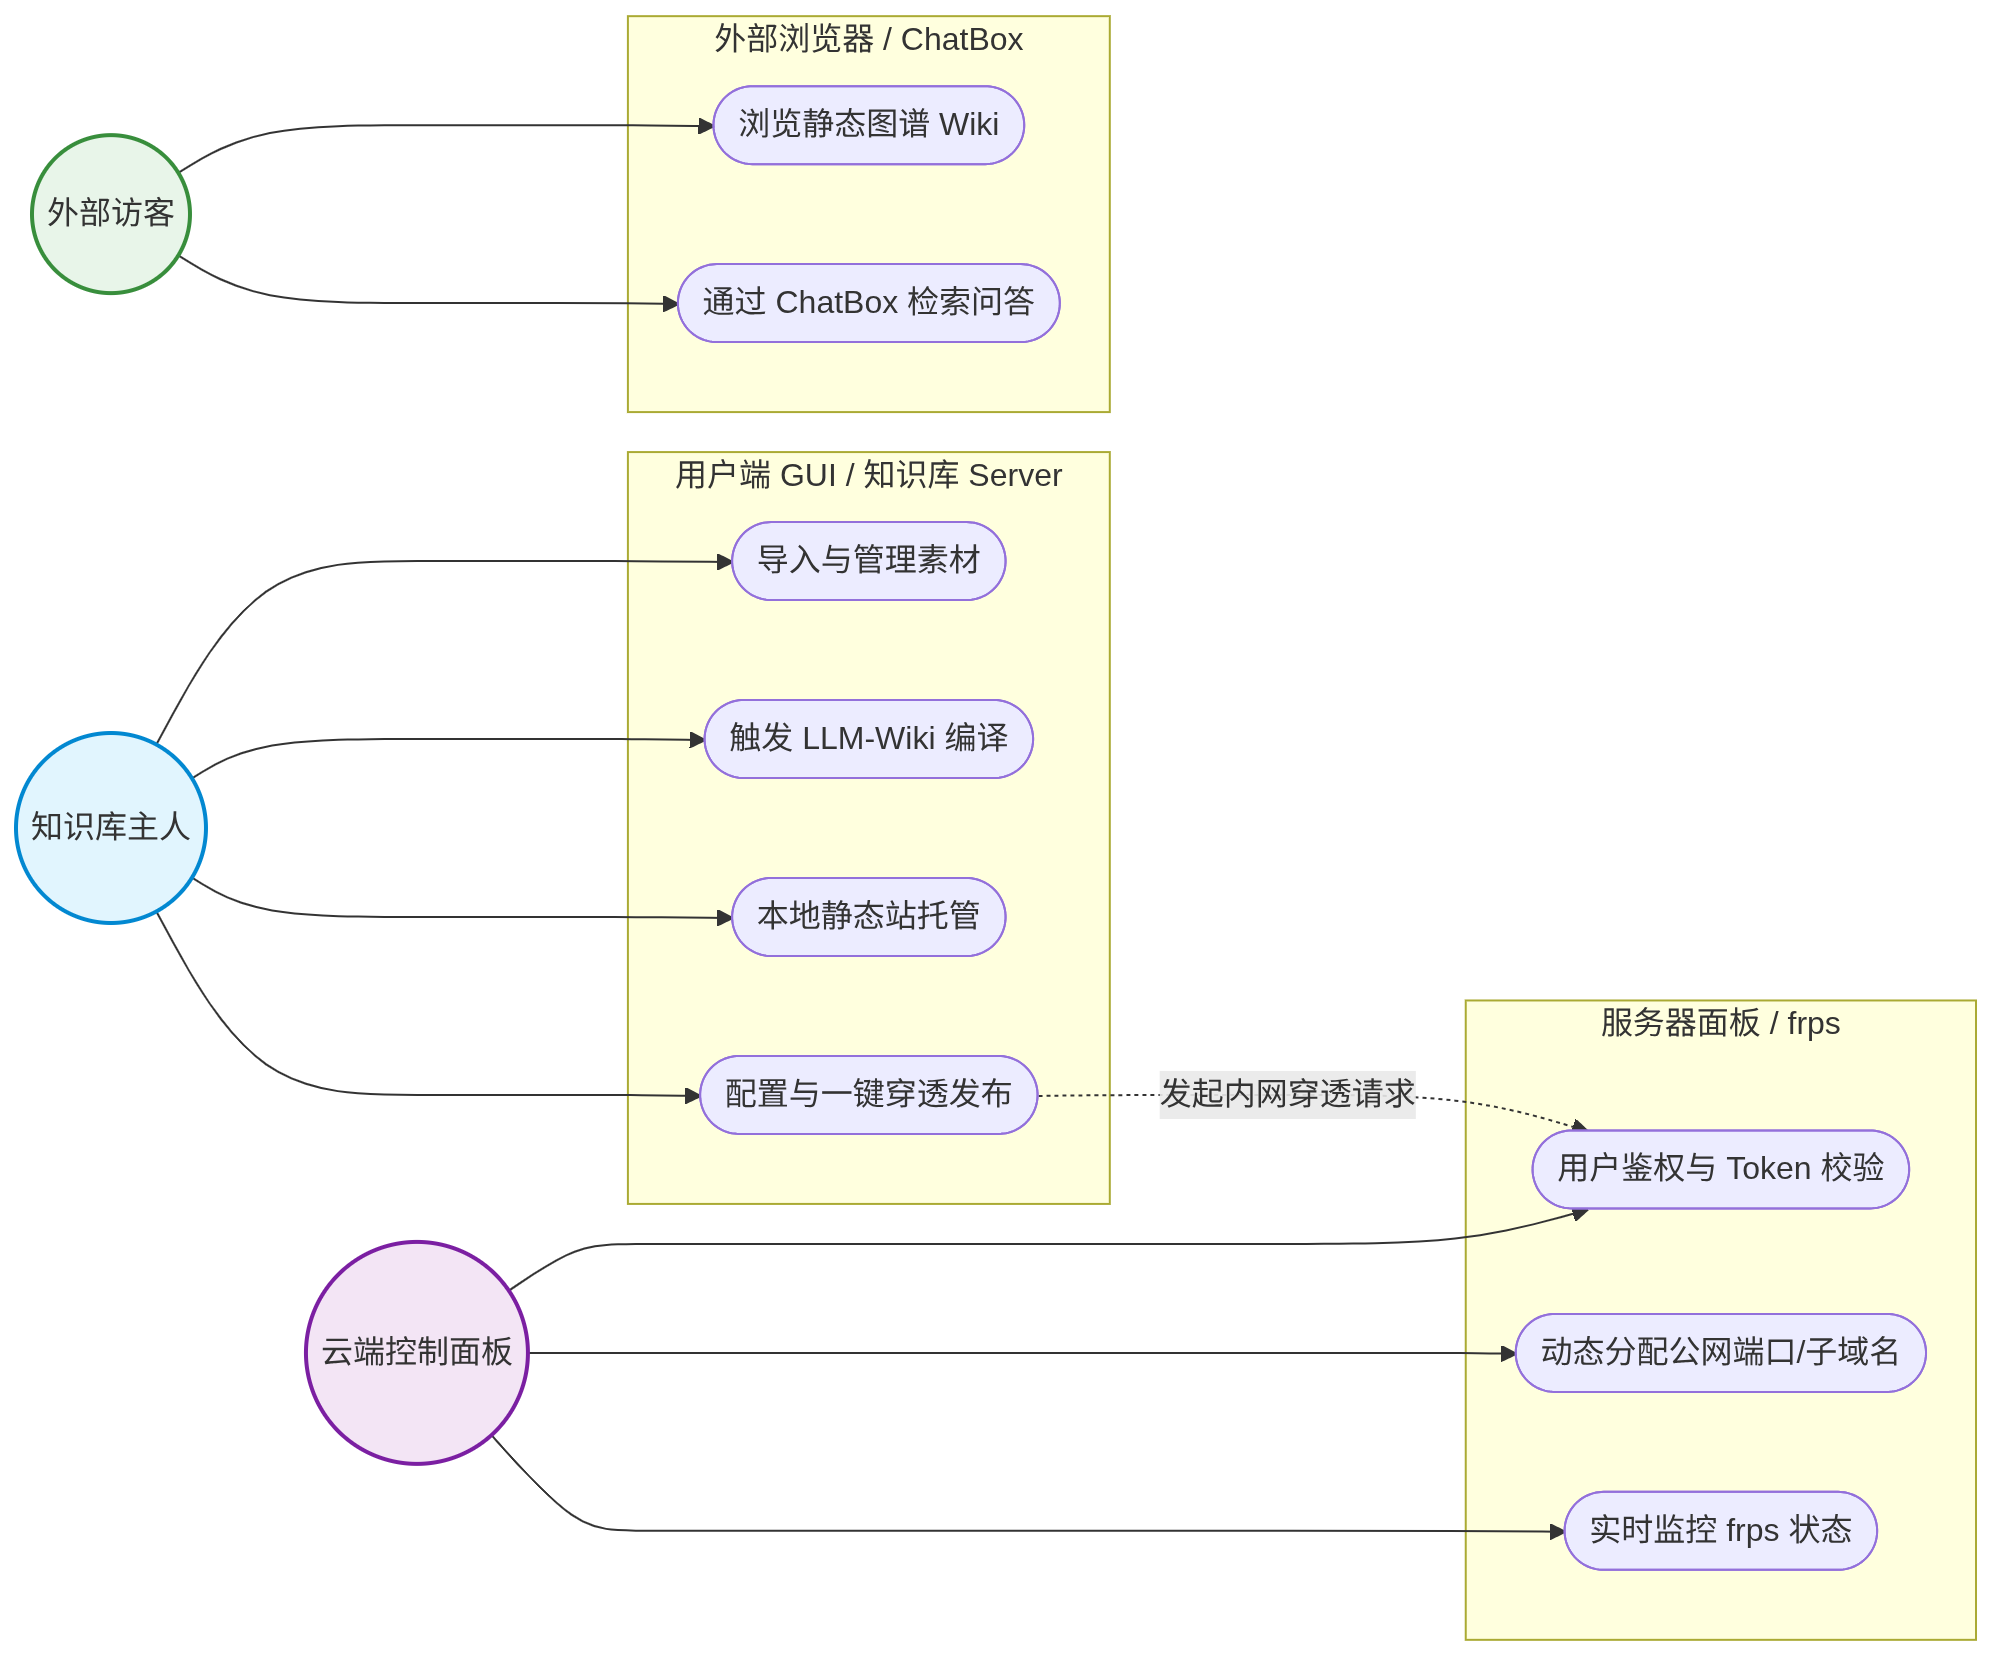
\includegraphics[width=0.86\textwidth]{image/usecase_diagram.png}
  \caption{WikiBridge 用例图：角色与系统边界}
  \label{fig:usecase}
\end{figure}

\noindent 图~\ref{fig:seq-overall} 给出端到端的发布与访问总流程（素材输入 → 本地编译 → frp 发布 →
浏览器消费）。

\begin{figure}[H]
  \centering
  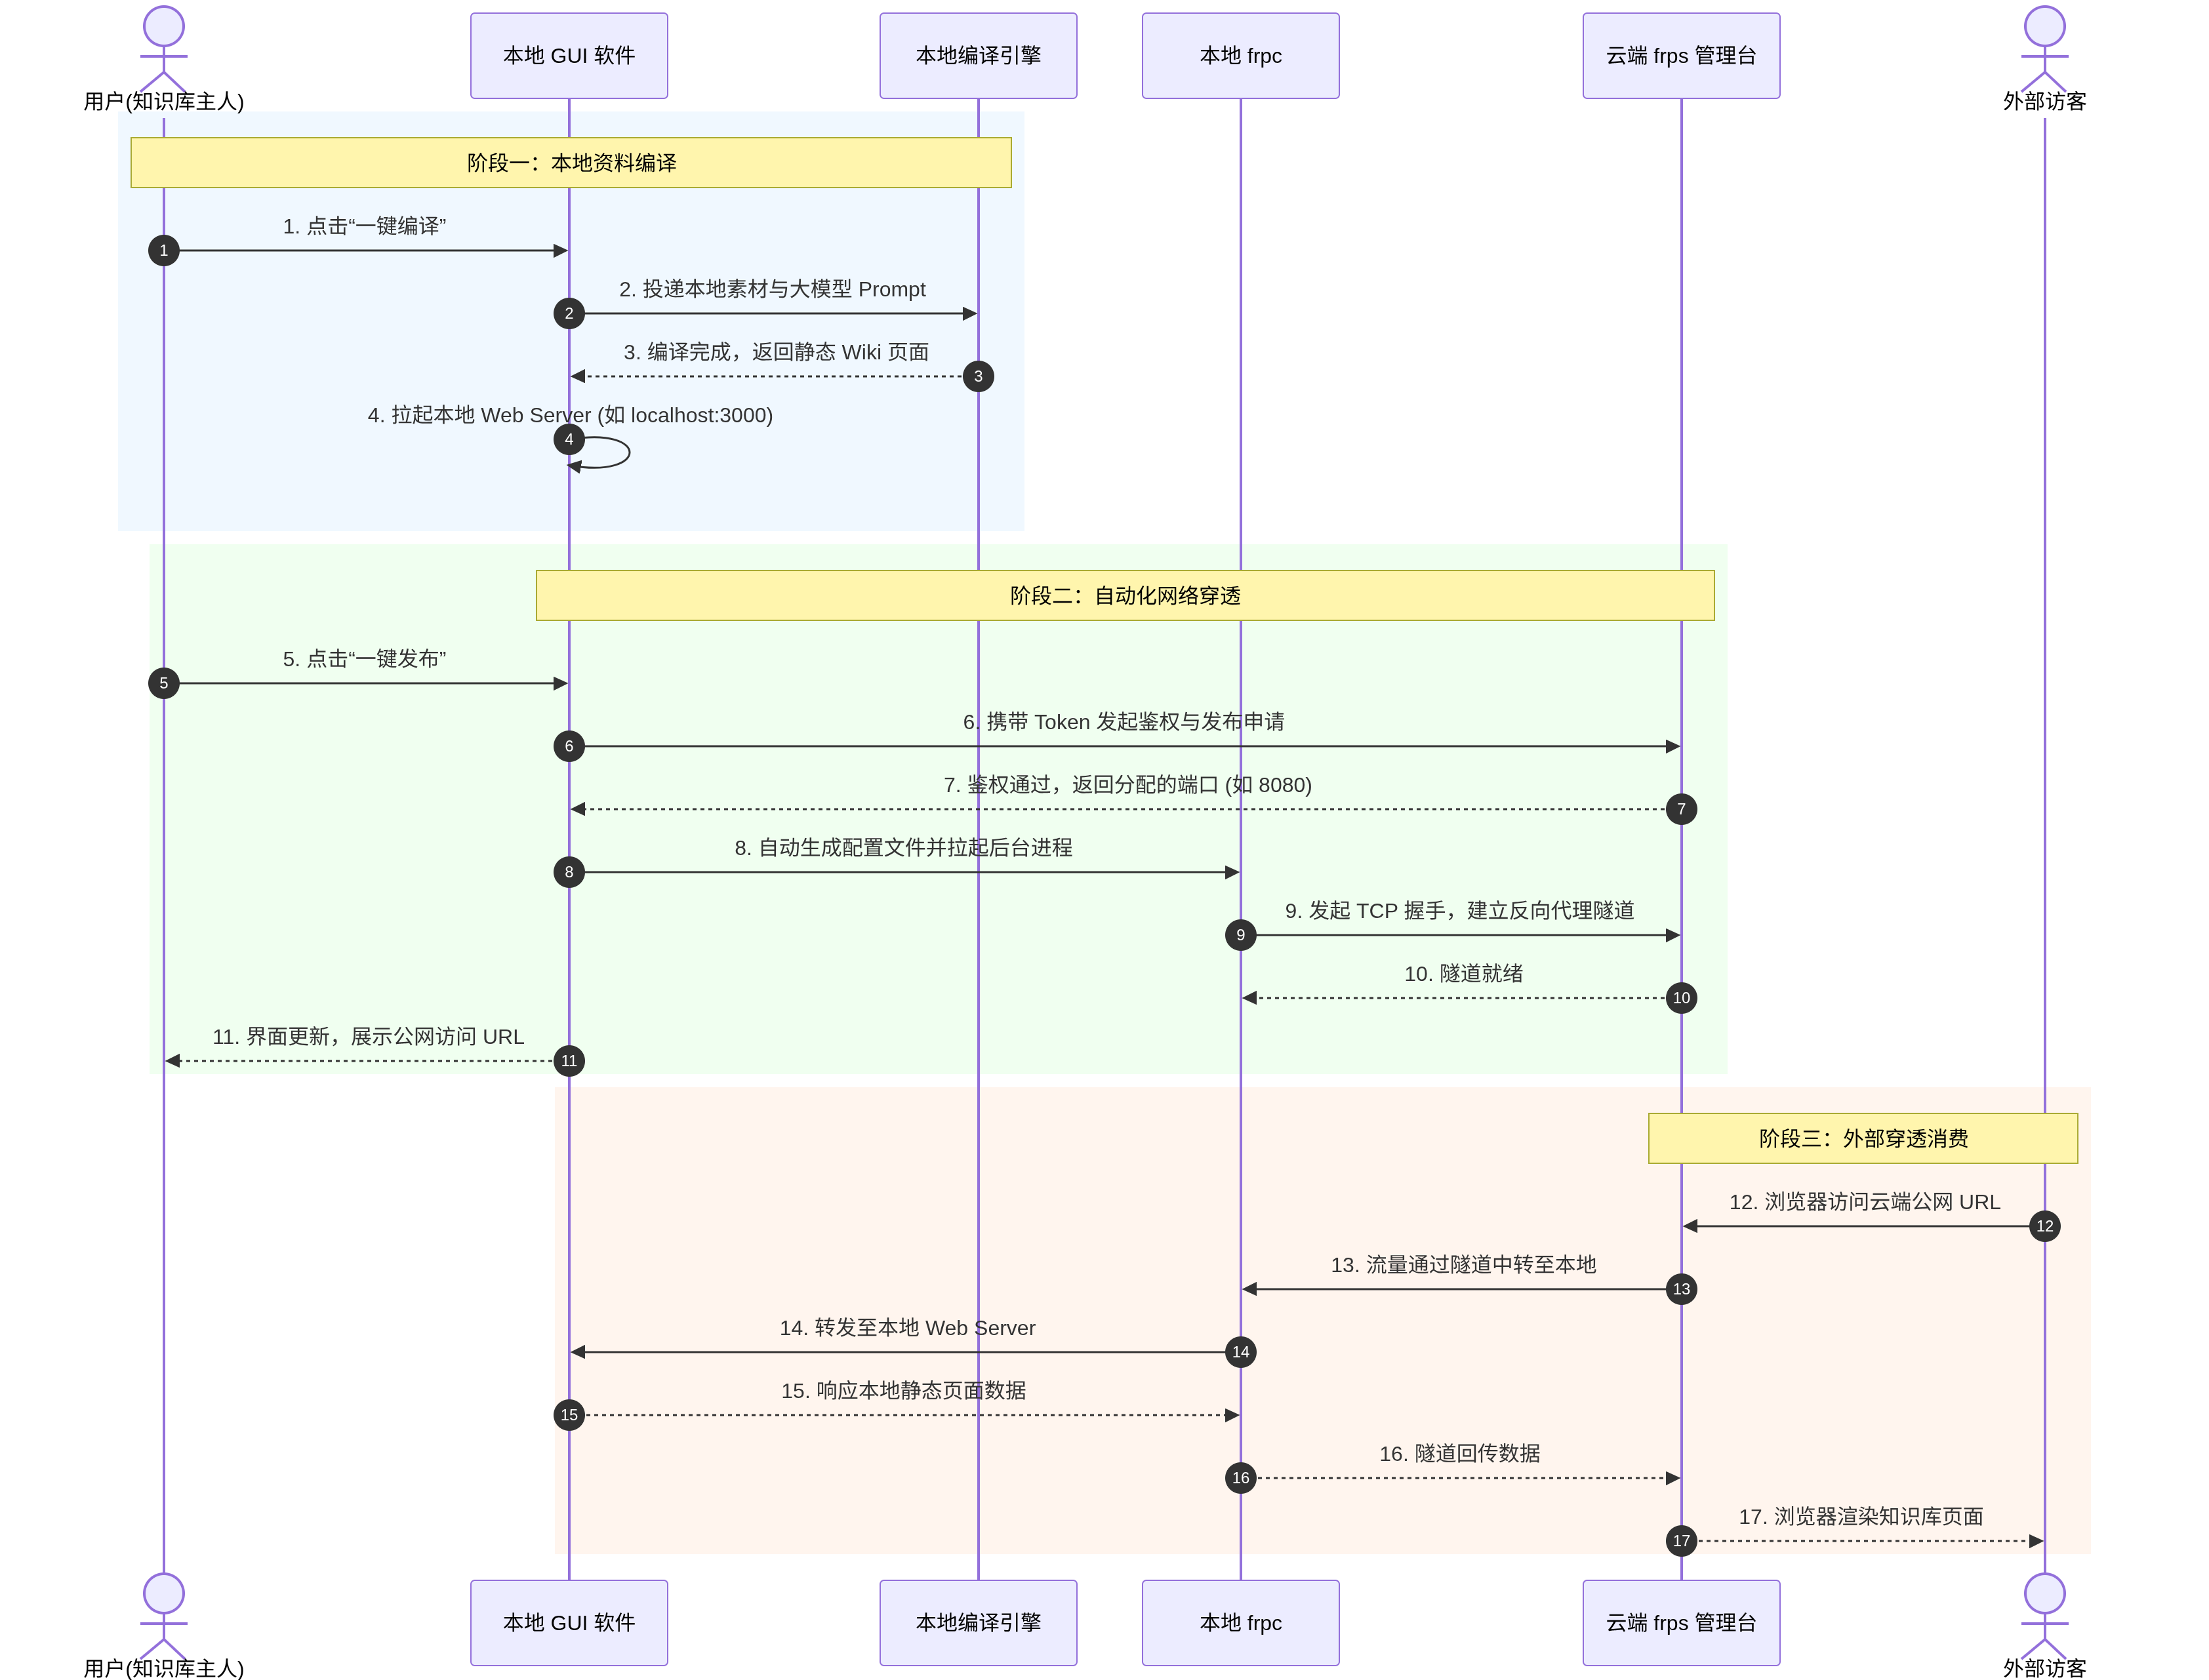
\includegraphics[width=0.92\textwidth]{image/sequence_diagram.png}
  \caption{端到端发布与访问流程顺序图}
  \label{fig:seq-overall}
\end{figure}

\noindent\textbf{（1）“Compile 本地编译”用例实现的设计方案}\quad
用户点击“开始编译”后，\code{CompileConsoleUI} 向控制类 \code{CompileManager} 发送
\code{startCompile()}；\code{CompileManager} 先扫描 \code{/raw} 中的新素材，随后调用
\code{LLMAgentClient} 的 \code{extractKnowledge(rawDocs)} 完成阅读、实体提取与去重，得到结构化结果后
交由 \code{WikiRepository} 的 \code{writePages()} 写入或合并 \code{/wiki} 中的 Markdown 页面并建立
\code{[[wiki-links]]}，最终把进度与日志反馈给界面。具体过程见图~\ref{fig:seq-compile}。

\begin{figure}[H]
  \centering
  \resizebox{\textwidth}{!}{%
  \begin{tikzpicture}[font=\sffamily]
    \def\yt{0}\def\yb{-7.0}
    \foreach \x/\name/\sty in {0/{用户}/actor, 2.8/{CompileConsoleUI}/obj, 6.2/{CompileManager}/obj,
        9.8/{LLMAgentClient}/obj, 13.0/{WikiRepository}/obj, 16.0/{/wiki 目录}/obj}{
      \node[\sty] at (\x,\yt) {\name};
      \draw[life] (\x,\yt-0.4) -- (\x,\yb);
    }
    \def\m#1#2#3#4{\draw[msg] (#1,#3) -- (#2,#3) node[slbl]{#4};}
    \def\r#1#2#3#4{\draw[ret] (#1,#3) -- (#2,#3) node[slbl]{#4};}
    \m{0}{2.8}{-0.9}{点击“开始编译”}
    \m{2.8}{6.2}{-1.5}{startCompile()}
    \draw[msg] (6.2,-2.1) -- ++(1.2,0) -- ++(0,-0.5) -- ++(-1.2,0);
    \node[font=\scriptsize\sffamily, anchor=west] at (7.5,-2.1) {scanRaw(/raw)};
    \m{6.2}{9.8}{-3.2}{extractKnowledge(rawDocs)}
    \r{9.8}{6.2}{-3.9}{entities, summaries}
    \m{6.2}{13.0}{-4.5}{writePages(structuredKB)}
    \m{13.0}{16.0}{-5.1}{写入/合并 Markdown + [[links]]}
    \r{16.0}{13.0}{-5.6}{ok}
    \r{13.0}{6.2}{-6.1}{writeResult}
    \r{6.2}{2.8}{-6.6}{进度 / 日志 / 完成}
  \end{tikzpicture}}
  \caption{“Compile 本地编译”用例实现的顺序图}
  \label{fig:seq-compile}
\end{figure}

\noindent\textbf{（2）“Publish 公网发布”用例实现的设计方案}\quad
用户登录后点击“发布”，\code{PublishPanelUI} 经 \code{AuthClient} 向服务器 \code{AuthController} 提交
账号密码并取得 Token；随后 \code{PublishManager} 启动本地 \code{LocalWebServer} 渲染 \code{/wiki}，并
驱动魔改 \code{frpc} 携带 Token 向 \code{TunnelController} 申请隧道；服务器分配子域名/端口并配置
\code{FrpsManager}，frpc 与 frps 建立隧道后回传公网 URL，界面最终向用户展示该 URL。具体过程见
图~\ref{fig:seq-publish}。

\begin{figure}[H]
  \centering
  \resizebox{\textwidth}{!}{%
  \begin{tikzpicture}[font=\sffamily]
    \def\yt{0}\def\yb{-7.4}
    \foreach \x/\name/\sty in {0/{用户}/actor, 2.6/{PublishPanelUI}/obj, 5.8/{frpc}/obj,
        9.0/{TunnelController}/obj, 12.2/{FrpsManager}/obj, 15.4/{消费端浏览器}/actor}{
      \node[\sty] at (\x,\yt) {\name};
      \draw[life] (\x,\yt-0.4) -- (\x,\yb);
    }
    \def\m#1#2#3#4{\draw[msg] (#1,#3) -- (#2,#3) node[slbl]{#4};}
    \def\r#1#2#3#4{\draw[ret] (#1,#3) -- (#2,#3) node[slbl]{#4};}
    \m{0}{2.6}{-0.9}{登录并点击“发布”}
    \m{2.6}{9.0}{-1.5}{login(account, password)}
    \r{9.0}{2.6}{-2.1}{token}
    \m{2.6}{5.8}{-2.7}{start(token, localPort)}
    \m{5.8}{9.0}{-3.3}{requestTunnel(token)}
    \r{9.0}{5.8}{-3.9}{subdomain / port}
    \m{5.8}{12.2}{-4.5}{establishTunnel(config)}
    \r{12.2}{5.8}{-5.1}{connected}
    \r{5.8}{2.6}{-5.7}{public URL}
    \r{2.6}{0}{-6.2}{展示公网 URL}
    \m{15.4}{12.2}{-6.8}{GET https://alice.wikibridge.app}
    \m{12.2}{5.8}{-7.2}{转发到本地 :localPort}
  \end{tikzpicture}}
  \caption{“Publish 公网发布”用例实现的顺序图}
  \label{fig:seq-publish}
\end{figure}

\noindent 图~\ref{fig:class-client} 给出“用户端”子系统的设计类图：在分析类的基础上，依据用例实现的
交互图增加了 \code{LLMAgentClient}、\code{WikiRepository}、\code{LocalWebServer}、\code{FrpcController}
等设计类，以实现知识编译与公网发布。

\begin{figure}[H]
  \centering
  \resizebox{0.98\textwidth}{!}{%
  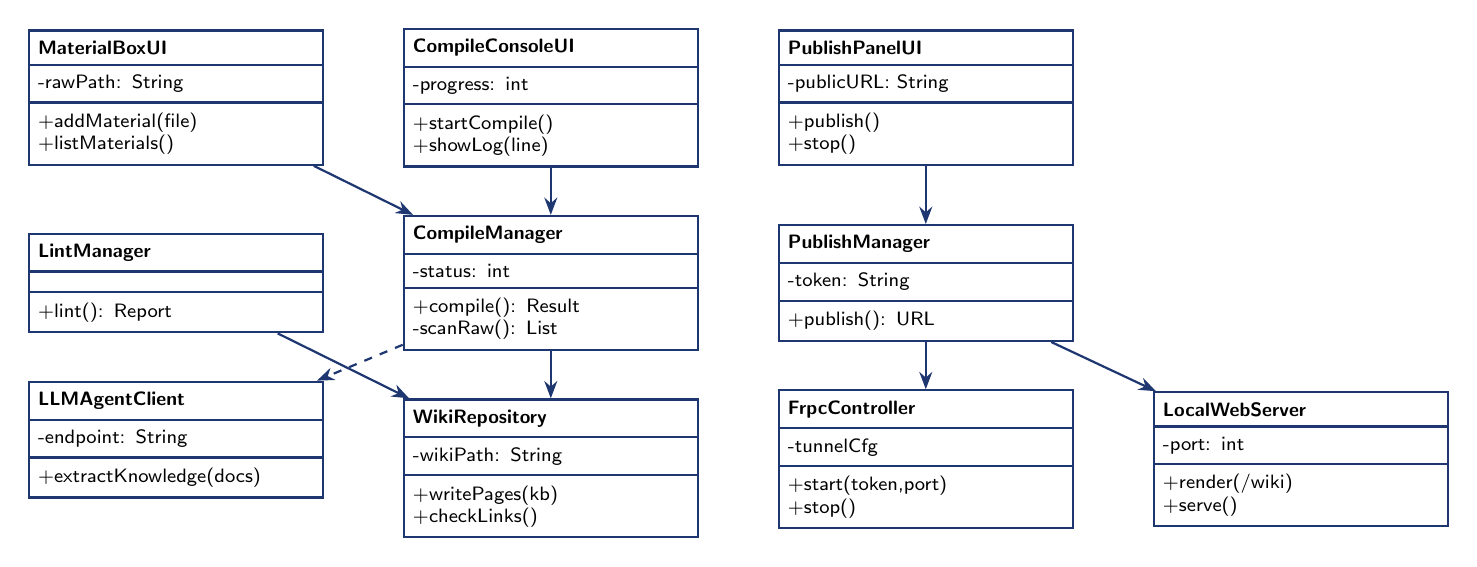
\begin{tikzpicture}[font=\sffamily, node distance=0.6cm and 1.0cm]
    \node[class] (matui) {\textbf{MaterialBoxUI}
      \nodepart{second}-rawPath: String
      \nodepart{third}+addMaterial(file)\\+listMaterials()};
    \node[class, right=of matui] (compui) {\textbf{CompileConsoleUI}
      \nodepart{second}-progress: int
      \nodepart{third}+startCompile()\\+showLog(line)};
    \node[class, right=of compui] (pubui) {\textbf{PublishPanelUI}
      \nodepart{second}-publicURL: String
      \nodepart{third}+publish()\\+stop()};

    \node[class, below=of compui] (cm) {\textbf{CompileManager}
      \nodepart{second}-status: int
      \nodepart{third}+compile(): Result\\-scanRaw(): List};
    \node[class, left=of cm] (lm) {\textbf{LintManager}
      \nodepart{second}
      \nodepart{third}+lint(): Report};
    \node[class, right=of cm] (pm) {\textbf{PublishManager}
      \nodepart{second}-token: String
      \nodepart{third}+publish(): URL};

    \node[class, below=of lm] (llm) {\textbf{LLMAgentClient}
      \nodepart{second}-endpoint: String
      \nodepart{third}+extractKnowledge(docs)};
    \node[class, below=of cm] (wiki) {\textbf{WikiRepository}
      \nodepart{second}-wikiPath: String
      \nodepart{third}+writePages(kb)\\+checkLinks()};
    \node[class, below=of pm] (frpc) {\textbf{FrpcController}
      \nodepart{second}-tunnelCfg
      \nodepart{third}+start(token,port)\\+stop()};
    \node[class, right=of frpc] (web) {\textbf{LocalWebServer}
      \nodepart{second}-port: int
      \nodepart{third}+render(/wiki)\\+serve()};

    \draw[flow] (matui) -- (cm);
    \draw[flow] (compui) -- (cm);
    \draw[flow] (pubui) -- (pm);
    \draw[dashedflow] (cm) -- (llm);
    \draw[flow] (cm) -- (wiki);
    \draw[flow] (lm) -- (wiki);
    \draw[flow] (pm) -- (frpc);
    \draw[flow] (pm) -- (web);
  \end{tikzpicture}}
  \caption{“用户端”子系统的设计类图}
  \label{fig:class-client}
\end{figure}

\noindent 图~\ref{fig:class-server} 给出“服务器（控制面）”子系统的设计类图。
\code{AuthController}、\code{TunnelController} 等控制类与 \code{UserRepository}、
\code{TunnelRepository} 实体类协作，完成认证、端口分配与状态持久化。

\begin{figure}[H]
  \centering
  \resizebox{0.92\textwidth}{!}{%
  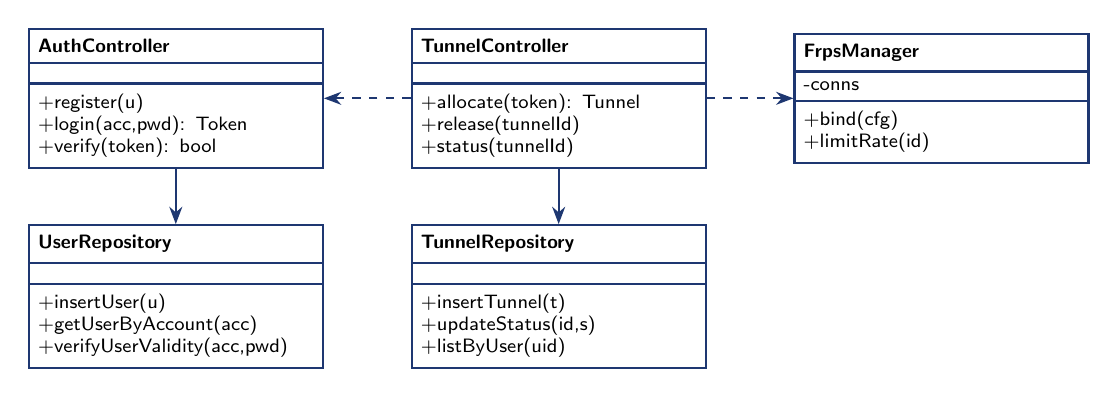
\begin{tikzpicture}[font=\sffamily, node distance=0.7cm and 1.1cm]
    \node[class] (authc) {\textbf{AuthController}
      \nodepart{second}
      \nodepart{third}+register(u)\\+login(acc,pwd): Token\\+verify(token): bool};
    \node[class, right=of authc] (tunc) {\textbf{TunnelController}
      \nodepart{second}
      \nodepart{third}+allocate(token): Tunnel\\+release(tunnelId)\\+status(tunnelId)};
    \node[class, right=of tunc] (frps) {\textbf{FrpsManager}
      \nodepart{second}-conns
      \nodepart{third}+bind(cfg)\\+limitRate(id)};

    \node[class, below=of authc] (userrepo) {\textbf{UserRepository}
      \nodepart{second}
      \nodepart{third}+insertUser(u)\\+getUserByAccount(acc)\\+verifyUserValidity(acc,pwd)};
    \node[class, below=of tunc] (tunrepo) {\textbf{TunnelRepository}
      \nodepart{second}
      \nodepart{third}+insertTunnel(t)\\+updateStatus(id,s)\\+listByUser(uid)};

    \draw[flow] (authc) -- (userrepo);
    \draw[flow] (tunc) -- (tunrepo);
    \draw[dashedflow] (tunc) -- (frps);
    \draw[dashedflow] (tunc) -- (authc);
  \end{tikzpicture}}
  \caption{“服务器（控制面）”子系统的设计类图}
  \label{fig:class-server}
\end{figure}

\subsection{核心流程设计}
WikiBridge 的主流程由用户主动触发的 \keypoint{Add / Compile / Lint / Publish} 四个阶段串联而成，
如图~\ref{fig:workflow} 所示。用户先把原始资料放入本地 \code{/raw}（Add），点击编译后由 LLM-Wiki
编译器读取新素材、提炼去重并写入 \code{/wiki}（Compile）；Lint 检查器扫描 \code{/wiki} 修复死链接与
冗余并\keypoint{写回}；本地 Web Server 将 \code{/wiki} 渲染为静态站点，用户确认发布后经 frp 隧道映射为
公网 URL（Publish），外部访问者即可在浏览器中浏览 Wiki 并使用 Chatbox 问答。该流程清晰地区分了
\keypoint{本地数据面}（Add/Compile/Lint/本地渲染）与\keypoint{公网发布}（Publish），普通浏览不触发
任何 Token 消耗。

\begin{figure}[H]
  \centering
  \resizebox{0.94\textwidth}{!}{%
  \begin{tikzpicture}[font=\sffamily\small,
    processbox/.style={draw=whu, thick, rounded corners=4pt, fill=white, align=center,
      minimum width=3.2cm, minimum height=1.0cm},
    dbox/.style={draw=whu, thick, cylinder, shape border rotate=90, aspect=0.24, fill=softgray,
      align=center, minimum height=0.9cm, minimum width=2.0cm},
    branch/.style={draw=whu, thick, diamond, fill=external, align=center, aspect=2.0, inner sep=1pt}]
    \node[processbox] (add) at (0,0) {Add\\加入本地素材};
    \node[dbox] (raw) at (3.3,0) {\code{/raw}\\原始资料};
    \node[processbox] (compile) at (6.6,0) {Compile\\LLM-Wiki 编译};
    \node[dbox] (wiki) at (9.9,0) {\code{/wiki}\\Markdown 页面};
    \node[processbox] (lint) at (13.2,0) {Lint\\图谱检查优化};

    \node[processbox] (web) at (6.6,-2.2) {本地 Web Server\\渲染静态站};
    \node[branch] (pub) at (9.9,-2.2) {是否\\发布};
    \node[processbox] (frp) at (13.2,-2.2) {Publish\\frp 公网映射};
    \node[processbox] (visit) at (16.5,-2.2) {浏览器访问\\Wiki / Chatbox};

    \draw[flow] (add) -- (raw);
    \draw[flow] (raw) -- (compile);
    \draw[flow] (compile) -- (wiki);
    \draw[flow] (wiki) -- (lint);
    \draw[flow] (wiki) -- (web);
    \draw[flow] (web) -- (pub);
    \draw[flow] (pub) -- node[lbl,above]{是} (frp);
    \draw[flow] (frp) -- (visit);
    \draw[flow] (lint.south) |- node[lbl,right]{修复后写回} (wiki.south);
  \end{tikzpicture}}
  \caption{Add / Compile / Lint / Publish 核心流程图}
  \label{fig:workflow}
\end{figure}

\subsection{类设计}
\noindent\textbf{（1）精化关键设计类间的关系}\quad
在分析类图中，\code{User}、\code{Token}、\code{TunnelConfig}、\code{WikiPage} 等类在设计阶段仍然有意义，
成为关键设计类。其关系精化见图~\ref{fig:class-rel}：一个 \code{User} 可持有多个 \code{Token}（一对多），
一个 \code{User} 可创建多个 \code{TunnelConfig}（一对多）；\code{WikiPage} 通过 \code{[[wiki-links]]} 与其它
\code{WikiPage} 形成自关联（多对多），由 \code{WikiRepository} 统一管理。

\begin{figure}[H]
  \centering
  \begin{tikzpicture}[font=\sffamily,
      ent/.style={draw=whu, thick, rounded corners=2pt, fill=client, align=center,
        minimum width=2.7cm, minimum height=0.9cm, font=\small\sffamily}]
    \node[ent] (user)   at (0,0)      {User};
    \node[ent] (token)  at (4.0,1.4)  {Token};
    \node[ent] (tunnel) at (4.0,-1.4) {TunnelConfig};
    \node[ent] (wiki)   at (8.6,0)    {WikiPage};
    \node[ent, fill=server] (repo) at (8.6,-2.4) {WikiRepository};

    \draw[thick,draw=whu] (user) -- node[lbl,pos=0.12,above]{1} node[lbl,pos=0.9,above]{*} (token);
    \draw[thick,draw=whu] (user) -- node[lbl,pos=0.12,below]{1} node[lbl,pos=0.9,below]{*} (tunnel);
    \draw[thick,draw=whu] (wiki.north)
      .. controls +(120:1.4) and +(60:1.4) .. (wiki.north);
    \node[lbl, above=0.95cm of wiki] {*\ \ [[link]]\ \ *};
    \draw[thick,draw=whu] (repo) -- node[lbl,right]{1\ \ 管理\ \ *} (wiki);
  \end{tikzpicture}
  \caption{精化关键设计类间的关系}
  \label{fig:class-rel}
\end{figure}

\noindent\textbf{（2）精化关键类属性的设计}\quad
关键设计类的属性精化见表~\ref{tab:attr}。所有用户私有信息（如密码、Token）可见范围均为
\code{private}，对外仅通过受控方法访问。

\begin{table}[H]
  \centering\small
  \caption{关键设计类的属性精化}
  \label{tab:attr}
  \begin{tabularx}{\textwidth}{l l l Y}
    \toprule
    \textbf{类} & \textbf{属性} & \textbf{类型 / 可见性} & \textbf{说明}\\
    \midrule
    User        & account   & String / private  & 用户账号，初值为空串\\
                & password  & String / private  & 用户密码，初值为空串\\
    Token       & value     & String / private  & 鉴权令牌，frpc 凭此申请隧道\\
                & expireAt  & long / private    & 过期时间戳\\
    TunnelConfig& subdomain & String / private  & 分配的子域名\\
                & localPort & int / private     & 本地服务端口\\
                & status    & int / private     & 隧道状态：IDLE/CONNECTED/CLOSED\\
    WikiPage    & title     & String / private  & 页面标题，唯一\\
                & links     & List<String> / private & 指向其它页面的 \code{[[wiki-links]]}\\
    \bottomrule
  \end{tabularx}
\end{table}

\noindent\textbf{（3）精化关键类方法的设计}\quad
关键控制类与实体类的方法签名精化见表~\ref{tab:method}。

\begin{table}[H]
  \centering\small
  \caption{关键类方法的精化设计}
  \label{tab:method}
  \begin{tabularx}{\textwidth}{l l Y}
    \toprule
    \textbf{类} & \textbf{可见性} & \textbf{方法签名与功能}\\
    \midrule
    CompileManager    & public  & \code{Result compile()} —— 扫描 /raw、调用 LLM、写入 /wiki\\
                      & private & \code{List<Doc> scanRaw(String path)} —— 读取新增素材\\
    LintManager       & public  & \code{LintReport lint()} —— 检查死链接、孤立页面与冗余\\
    PublishManager    & public  & \code{String publish()} —— 启动本地服务并申请隧道，返回 URL\\
    LLMAgentClient    & public  & \code{KB extractKnowledge(List<Doc> docs)} —— 提炼结构化知识\\
    WikiRepository    & public  & \code{void writePages(KB kb)} / \code{bool checkLinks()}\\
    AuthController    & public  & \code{Token login(String acc, String pwd)} / \code{bool verify(Token t)}\\
    TunnelController  & public  & \code{Tunnel allocate(Token t)} / \code{void release(String id)}\\
    UserRepository    & public  & \code{bool verifyUserValidity(String acc, String pwd)}\\
    \bottomrule
  \end{tabularx}
\end{table}

\noindent\textbf{（4）构造类的状态图}\quad
\code{TunnelConfig}（发布隧道）对象在其生命周期中需针对外部事件（登录、断网、回收等）变迁状态，
因此为其构造状态图。图~\ref{fig:state} 描述了发布隧道从空闲、连接、在线服务到断线重连与关闭的
生命周期及容错路径。

\begin{figure}[H]
  \centering
  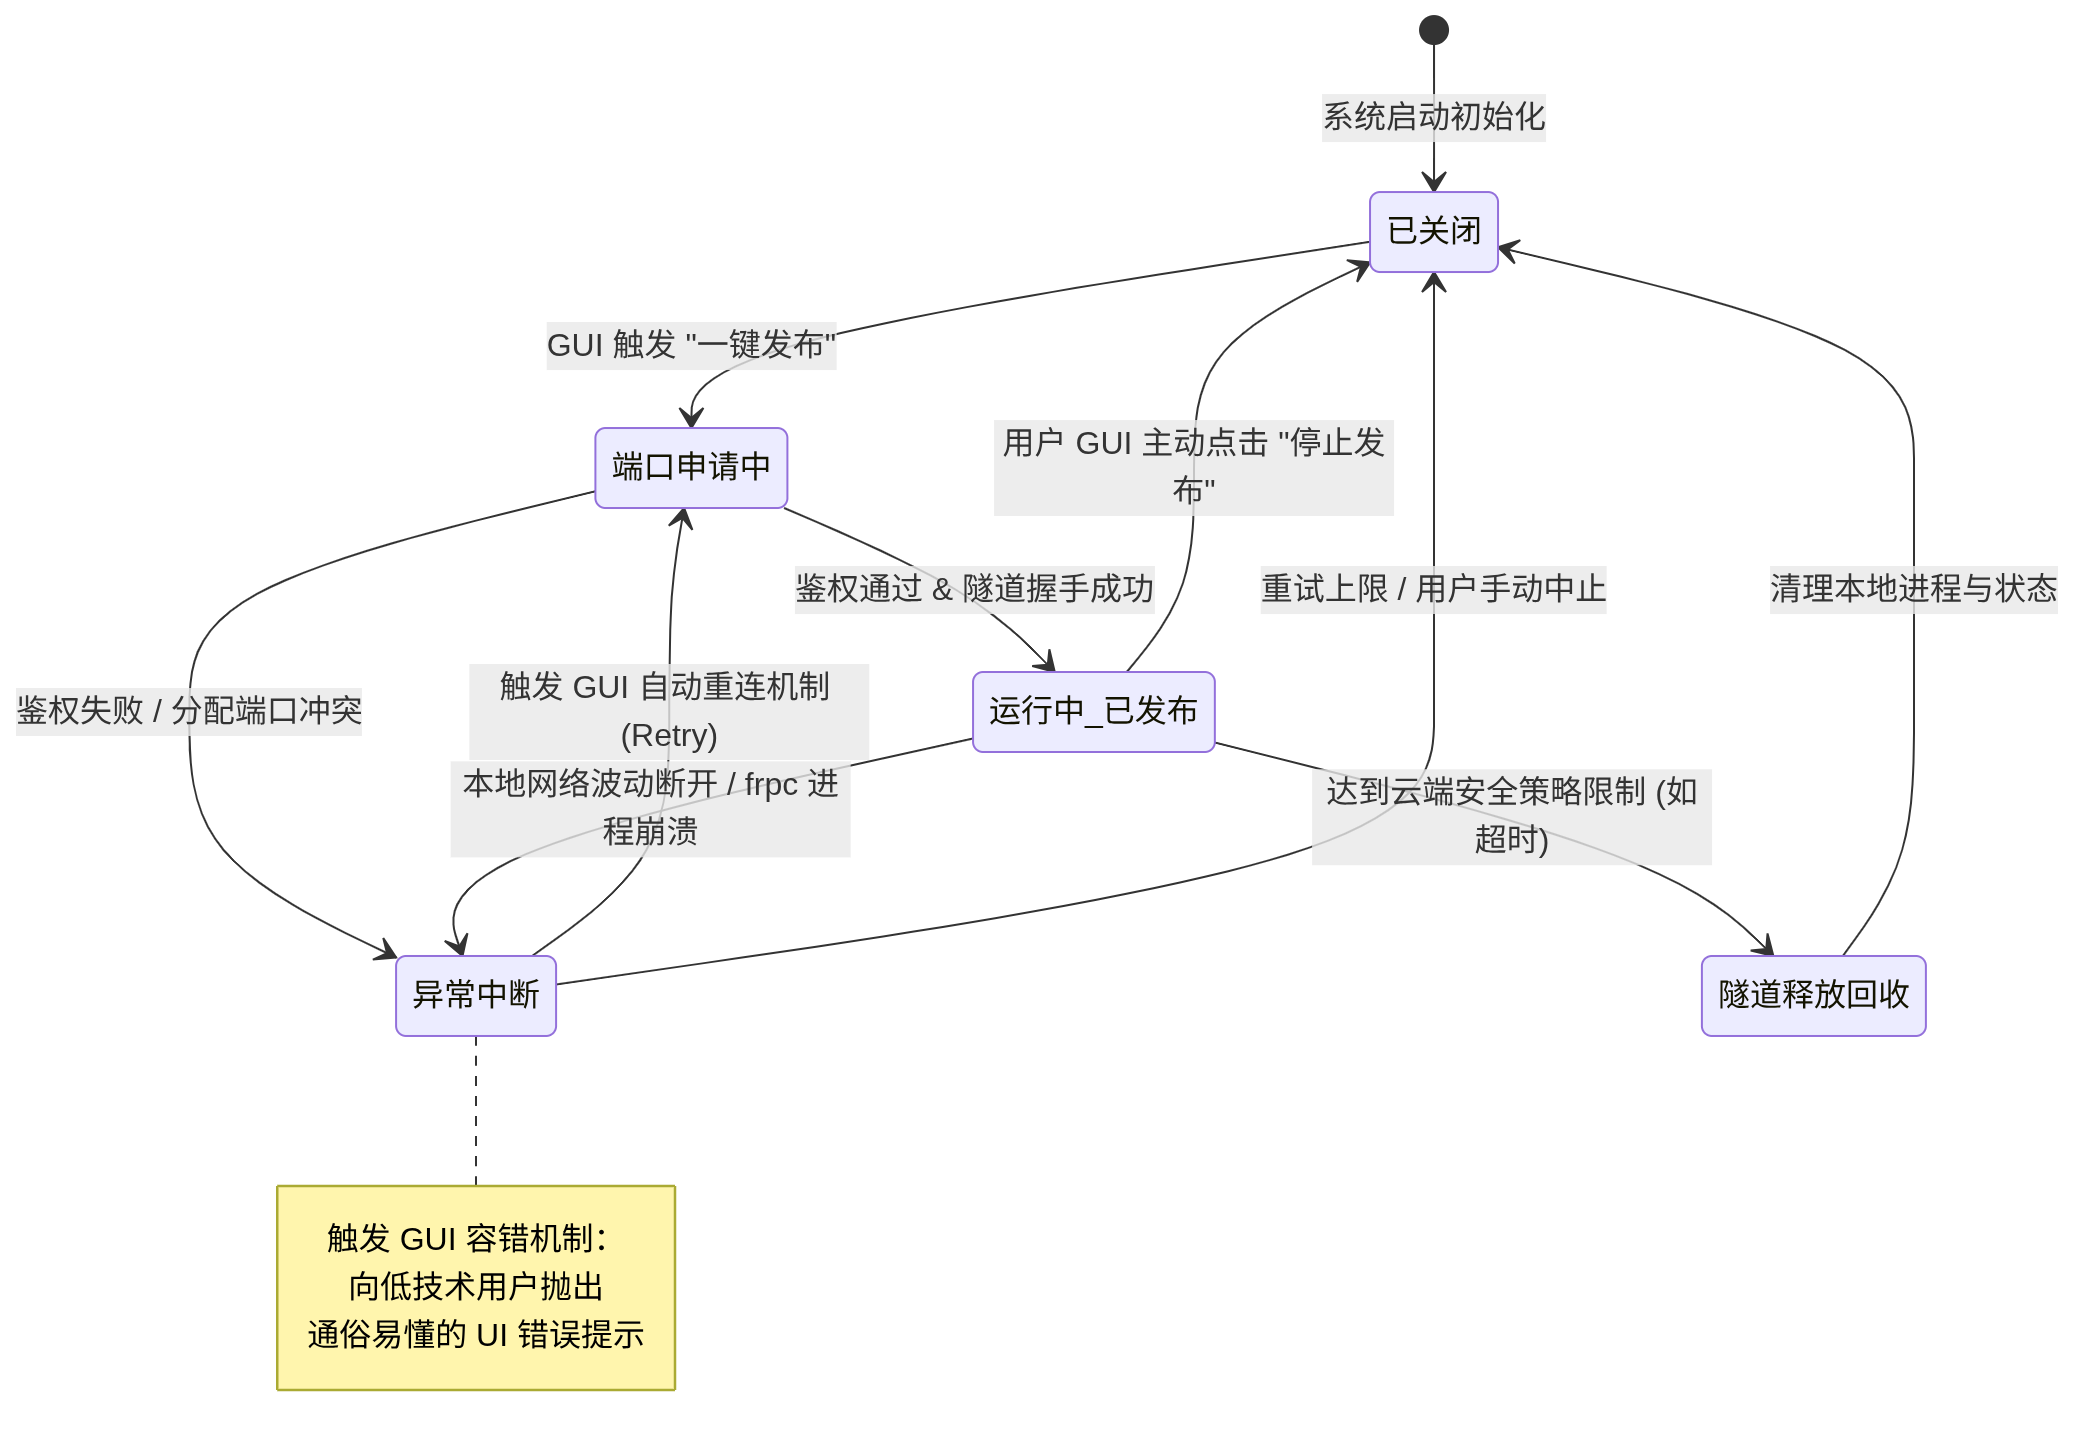
\includegraphics[width=\textwidth,height=0.6\textheight,keepaspectratio]{image/state_diagram.png}
  \caption{发布隧道（TunnelConfig）对象的状态图}
  \label{fig:state}
\end{figure}

\subsection{数据设计}
WikiBridge 的数据分为\keypoint{本地数据}与\keypoint{服务器控制面数据}两部分。系统\keypoint{明确避免}
把用户知识内容上传到服务器持久化保存：用户原始资料、Wiki 页面、本地索引与问答上下文均保留在本地，
服务器只保存账号、Token、发布记录与隧道状态，以此满足非功能性需求中的隐私与安全约束。

\subsubsection{本地数据结构}
用户端在用户选定的工作目录下初始化并维护以下本地数据，见表~\ref{tab:localdata}。

\begin{table}[H]
  \centering\small
  \caption{用户端本地数据结构}
  \label{tab:localdata}
  \begin{tabularx}{\textwidth}{l l Y}
    \toprule
    \textbf{路径 / 文件} & \textbf{数据内容} & \textbf{说明}\\
    \midrule
    \code{/raw}         & 原始资料           & 用户放入的 Word、PDF、网页摘录、笔记、Markdown、TXT 等。\\
    \code{/wiki}        & Markdown Wiki 页面 & 编译后的结构化页面，含标题、正文、标签与 \code{[[wiki-links]]}。\\
    \code{/index}       & 本地索引           & 供搜索与 Chatbox 使用的全文 / 向量 / 摘要索引。\\
    \code{config.json}  & 本地配置           & 素材目录、Wiki 目录、本地端口、模型配置、发布偏好。\\
    \code{material.db}  & 素材状态           & 文件路径、哈希、更新时间、处理状态、失败原因。\\
    \code{publish.json} & 发布状态缓存       & 当前公网 URL、隧道状态、最近连接时间与可回收标识。\\
    \bottomrule
  \end{tabularx}
\end{table}

\subsubsection{服务器控制面数据表}
服务器侧的核心数据库表（用户与隧道）及其关联见图~\ref{fig:db}：\code{T\_User} 保存用户账号信息，
\code{T\_Tunnel} 保存每次发布申请到的隧道与公网入口信息，二者通过 \code{user\_id} 关联。

\begin{figure}[H]
  \centering
  \resizebox{\textwidth}{!}{%
  \begin{tikzpicture}[font=\sffamily,
      tbl/.style={draw=whu, thick, rectangle split, rectangle split parts=2,
        rectangle split draw splits=true, fill=white, align=left, text width=5.2cm, font=\scriptsize\sffamily}]
    \node[tbl] (u) {\textbf{T\_User}
      \nodepart{second}
      \underline{id : INT (PK)}\\
      account : VARCHAR(50)\\
      password : VARCHAR(64)\\
      type : INT\quad(用户类别)\\
      created\_at : DATETIME};
    \node[tbl, right=2.4cm of u] (t) {\textbf{T\_Tunnel}
      \nodepart{second}
      \underline{id : INT (PK)}\\
      user\_id : INT (FK)\\
      subdomain : VARCHAR(64)\\
      local\_port : INT\\
      status : INT\\
      public\_url : VARCHAR(128)\\
      connected\_at : DATETIME};
    \draw[thick,draw=whu] (u.east) -- node[lbl,above]{1} node[lbl,above,pos=0.9]{*} (t.west);
  \end{tikzpicture}}
  \caption{控制面数据库表 \code{T\_User} 与 \code{T\_Tunnel}}
  \label{fig:db}
\end{figure}

\noindent 为支撑认证、发布、状态监控与防滥用，服务器侧完整的控制面数据表设计见表~\ref{tab:servertables}，
所有表均\keypoint{不含}任何用户知识内容。

\begin{longtable}{>{\bfseries\ttfamily}p{3.4cm}p{10.6cm}}
  \caption{服务器控制面数据表设计}\label{tab:servertables}\\
  \toprule
  数据表 & 字段说明 \\
  \midrule\endfirsthead
  \toprule
  数据表 & 字段说明 \\
  \midrule\endhead
  T\_User          & \code{id}、\code{account}、\code{password\_hash}、\code{display\_name}、\code{status}、\code{created\_at}、\code{last\_login\_at}。保存平台账号，不保存知识内容。\\
  T\_AccessToken   & \code{id}、\code{user\_id}、\code{token\_hash}、\code{expire\_at}、\code{revoked\_at}。用于 Token 校验与吊销。\\
  T\_PublishRecord & \code{id}、\code{user\_id}、\code{subdomain}、\code{public\_port}、\code{local\_port}、\code{status}、\code{created\_at}、\code{closed\_at}。记录每次发布入口。\\
  T\_TunnelStatus  & \code{id}、\code{publish\_id}、\code{online}、\code{bandwidth\_in}、\code{bandwidth\_out}、\code{connection\_count}、\code{last\_heartbeat}。管理 frp 隧道运行状态。\\
  T\_RateLimitPolicy & \code{id}、\code{user\_id}、\code{max\_bandwidth}、\code{max\_connections}、\code{enabled}。基础限速与防滥用策略。\\
  \bottomrule
\end{longtable}

\subsubsection{永久数据的操作}
为支持对上述数据库表的操作，设计模型提供两个仓储类 \code{UserRepository} 与
\code{TunnelRepository}，其接口如下：
\begin{itemize}[leftmargin=2.2em, itemsep=1pt]
  \item \code{boolean insertUser(User u)} / \code{boolean deleteUser(User u)} / \code{boolean updateUser(User u)}
  \item \code{User getUserByAccount(String account)} / \code{boolean verifyUserValidity(String acc, String pwd)}
  \item \code{boolean insertTunnel(TunnelConfig t)} / \code{boolean updateStatus(String id, int status)}
  \item \code{List<TunnelConfig> listByUser(int userId)} / \code{void closeTunnel(String id)}
  \item \code{void openDatabase()} / \code{void closeDatabase()}
\end{itemize}

\subsubsection{数据安全设计}
为保护用户隐私与账号安全，数据设计遵循以下约束：
\begin{itemize}[leftmargin=2.2em, itemsep=1pt]
  \item 本地 \code{config.json} 中的 Token 应\keypoint{加密保存}或使用操作系统的安全存储能力，不以明文长期驻留。
  \item 日志中\keypoint{不得输出}完整 Token、用户密码、原始资料全文以及模型请求的完整上下文。
  \item 服务器侧密码仅保存\keypoint{哈希值}（\code{password\_hash}），Token 仅保存哈希或可验证摘要（\code{token\_hash}）。
  \item 发布入口支持用户主动关闭，管理员也可在滥用或异常流量场景下回收入口（\code{revoked\_at} / \code{closed\_at}）。
\end{itemize}

\subsection{部署设计}
WikiBridge 采用分布式部署（见图~\ref{fig:deploy}）。用户端软件（GUI、知识编译器、本地 Web Server、
魔改 frpc）部署在知识拥有者的个人主机上；服务器端（管理 API、frps、控制面数据库）部署在公网云
主机上；知识消费端为任意带浏览器的设备。用户端 frpc 与服务器 frps 之间通过 frp 隧道连接，消费端
浏览器经服务器公网入口被转发回用户端本地服务，从而在\keypoint{不暴露用户主机}的前提下完成访问。

\begin{figure}[H]
  \centering
  \resizebox{\textwidth}{!}{%
  \begin{tikzpicture}[font=\sffamily\small]
    \node[node3d, fill=client, align=left] (client) at (0,0)
      {\textbf{《device》用户主机}\\[3pt]
       \scriptsize · GUI 控制台\\ \scriptsize · 知识编译器 + LLM 客户端\\
       \scriptsize · 本地 Web Server :8080\\ \scriptsize · 魔改 frpc\\
       \scriptsize · 本地 /raw、/wiki};
    \node[node3d, fill=server, align=left, minimum height=2.6cm] (server) at (7,0)
      {\textbf{《device》云服务器（Linux）}\\[3pt]
       \scriptsize · 管理 API（认证/端口）\\ \scriptsize · frps 服务\\
       \scriptsize · 控制面数据库 MySQL\\ \scriptsize · 流量统计/限速};
    \node[node3d, fill=external, align=left, minimum height=1.8cm, minimum width=3.6cm] (browser) at (12.4,0)
      {\textbf{《device》消费端}\\[3pt]
       \scriptsize · 浏览器\\ \scriptsize · Wiki 浏览 + Chatbox};
    \draw[flow] (client.north) to[out=60,in=120] node[lbl,above]{frp 隧道（控制+数据）} (server.north);
    \draw[dashedflow] (client.south) to[out=-60,in=-120] node[lbl,below]{HTTPS 管理 API（登录/申请）} (server.south);
    \draw[flow] (browser) -- node[lbl,above]{HTTPS 公网入口} (server);
  \end{tikzpicture}}
  \caption{WikiBridge 系统的部署图}
  \label{fig:deploy}
\end{figure}

\subsection{异常处理与可靠性设计}
为满足非功能性需求中的可靠性，系统针对编译、网络与发布链路上的典型异常给出检测与处理策略，
见表~\ref{tab:exception}。设计原则是\keypoint{失败隔离、状态可见、可恢复}：单个素材或单次调用失败不应
阻塞整体流程，所有异常都应在界面给出可理解的提示而非仅输出底层日志。

\begin{longtable}{>{\bfseries}p{3.3cm}p{4.8cm}p{5.7cm}}
  \caption{异常处理与可靠性设计}\label{tab:exception}\\
  \toprule
  异常场景 & 检测方式 & 处理策略 \\
  \midrule\endfirsthead
  \toprule
  异常场景 & 检测方式 & 处理策略 \\
  \midrule\endhead
  素材解析失败   & 解析器返回错误或文本为空       & 标记素材失败，不阻塞其他素材编译，允许查看原因并重试。\\
  大模型调用失败 & 超时、限流、返回格式不合法     & 记录日志，按任务粒度重试，必要时保留半成品并提示用户。\\
  Wiki 链接异常  & Lint 扫描到死链接或孤立页面    & 给出修复建议，涉及删除或合并时等待用户确认。\\
  本地端口占用   & 本地 Web Server 启动失败       & 自动建议备用端口，并同步更新 frpc 配置。\\
  Token 过期     & 服务器返回未授权               & 提示重新登录，暂停发布操作但不影响本地浏览。\\
  隧道断开       & frpc 心跳或 frps 状态异常      & 自动重连并在界面展示状态；多次失败后提示检查网络。\\
  公网访问滥用   & 流量与连接数超过阈值           & 服务器限速、临时关闭入口或要求用户重新确认发布。\\
  \bottomrule
\end{longtable}

\subsection{测试设计}
课程设计原型阶段建议按以下端到端场景进行验收：
\begin{enumerate}[leftmargin=2.4em, itemsep=1pt]
  \item \keypoint{素材箱测试}：将多种格式资料加入 \code{/raw}，确认系统能识别新增素材并展示状态。
  \item \keypoint{编译测试}：触发 Compile 后生成多个 Markdown 页面，标题清晰且存在合理双向链接。
  \item \keypoint{图谱检查测试}：构造死链接、孤立页面和重复主题，确认 Lint 能识别并给出建议。
  \item \keypoint{本地浏览测试}：启动本地 Web Server 后，浏览器可打开 Wiki 首页、页面详情与搜索结果。
  \item \keypoint{发布测试}：登录后申请公网 URL，外部浏览器可通过该 URL 访问本地 Wiki。
  \item \keypoint{问答测试}：在 Chatbox 中提问，系统返回回答与引用来源，引用可跳转到对应页面。
  \item \keypoint{隐私测试}：检查服务器数据库与日志，确认未保存用户原始资料、Wiki 正文或问答上下文。
  \item \keypoint{异常测试}：模拟端口占用、网络断开、Token 过期与模型调用失败，确认界面提示清晰且可恢复。
\end{enumerate}

\section*{结论}
\addcontentsline{toc}{section}{结论}
WikiBridge 的设计目标是验证“\keypoint{LLM-Wiki 本地编译 + frp 无感穿透}”的端到端可行性。系统通过
\keypoint{控制面与数据面分离}、\keypoint{知识编译与 frp 管理解耦}两条主线，在三端架构下实现了“本地编译 +
无感穿透”的完整闭环：用户端承担知识内容处理与本地托管，服务器只承担认证、端口分配与隧道调度，消费端
以浏览器轻量浏览和问答。用户数据与主要计算过程留在本地，云端只做轻量调度，从而同时兼顾\keypoint{低门槛、
隐私性、低成本与可维护性}。后续实现应优先打通从本地素材到 Markdown Wiki、从本地 Web Server 到公网 URL 的
主链路，再逐步完善 Lint 自动修复、访问控制、限速策略与跨平台安装体验。

\end{document}
